\section{Metabolisme bag fysisk aktivitet}
Ved fysisk aktivitet kræver musklerne energi. Dette sker ved fraspaltning af en fosfatgruppe (P) fra adenosintrifosfat (ATP), som derefter bliver til adenosindifosfat (ADP). ATP skal derfor gendannes konstant, hvilket kan foregå under aerobe eller anaerobe forhold.\fxnote{Anaerob=uden ilt, aerob=med ilt} Under anaerobe forhold er der ikke tilstrækkelig ilt til stede, hvorfor denne proces er den første, som indtræder under fysisk aktivitet. ATP kan gendannes anaerobt ved spaltning af kreationfosfat eller kulhydrater under dannelse af mælkesyre. \\
Under aerobe forhold kan ATP gendannes i meget store mængder, hvorfor denne proces for alvor først dominerer efter cirka tyve minutter, som kan ses på \figref{fig:Metabolisme}. Denne proces kræver ADP, P, ilt og kulhydrat eller fedt til at gendanne ATP, vand og kuldioxid. Den areobe proces kan danne 12 gange mere ATP pr. gram kulhydrat i forhold til den anaerobe proces, men dette kan dog variere. Effektiviteten af den aerobe proces afhænger, hvor veltrænet kroppen er samt hvor gode musklerne er til at optage den tilførte ilt. 
\begin{figure}[H]
	\centering
	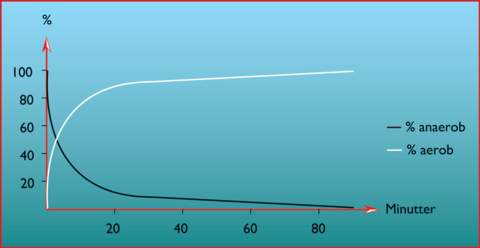
\includegraphics[scale=0.75]{figures/aProblemanalyse/Metabolisme.png}
	\caption{På figuren ses den procentvise fordeling af gendannelsesprocesserne af ATP. Der ses, at efter cirka 20 minutter overtager den aerobe proces, da der her dan}
	\label{fig:Metabolisme}
\end{figure}


Aerobt arbejde: er muskelarbejde hvor ilt kræves til fremskaffelsen af energi. De aerobe processer starter ved arbejdets start men domineres de første minutter af anaerobt arbejde, fordi kredsløbet først er i fulde omdrejninger efter ca. 4 min.

Hvor stort et aerobt arbejde man kan udføre, eller hvor høj intensitet man kan ligge med i længere tid, afgøres af hvor veltrænet ens kredsløb er (hjertets pumpeevne, lungernes volumen, blodmængden og musklernes evne til at forbrænde ilt i mitochondrierne).

Glykogen: Er et vigtigt energilager der kan forbrændes aerobt i muskelcellerne (mitochondrierne). Glykogenet dominerer de første 20 min. af et muskelarbejde og foretrækkes af muskelcellerne når intensiteten stiger. Et glykogenmolekyle giver 38 ATP.

Fedt: Er det andet energilager der indgår i forbrændingen i muskelcellen. Fedtforbrænding begynder først efter 20 -30 min. og fedtets andel i forbrændingen er størst ved lavere intensiteter.

%%%% KILDE: https://ibog-idraetc.systime.dk/index.php?id=90
%%%% https://idraetsteori.wikispaces.com/Aerob+energioms%C3%A6tning
%%% http://download.springer.com/static/pdf/163/art%253A10.1007%252FBF03345235.pdf?originUrl=http%3A%2F%2Flink.springer.com%2Farticle%2F10.1007%2FBF03345235&token2=exp=1456403695~acl=%2Fstatic%2Fpdf%2F163%2Fart%25253A10.1007%25252FBF03345235.pdf%3ForiginUrl%3Dhttp%253A%252F%252Flink.springer.com%252Farticle%252F10.1007%252FBF03345235*~hmac=08d77f7585b5cfaf4478d76647c53cccffd1b76fc44f2356e4379689dd95143e

%% Skrive: Skriv og søg lidt mere på anaerob og aerobe forhold hver for sig, så man går lidt mere i detaljer. Er der andre metabolske processer, som er vigtige?